\begin{center}\large\textbf{Readings: Chapter 3 (you can skip the guidelines for constructing class intervals, stem-and-leaf plots, grouped mean/median)}\\
\normalsize \end{center}
\large ~\hrulefill
~\\
\normalsize \\~\\
Recall:  Process of a study involves
\begin{enumerate}
\item Identify the research objective
\item Collect the information needed to answer the questions
\item Organize and summarize the information.
\item Draw conclusions from the information.
\end{enumerate}
We will now talk about step 3!\\~\\
So you have data... now what??\\
\begin{center}
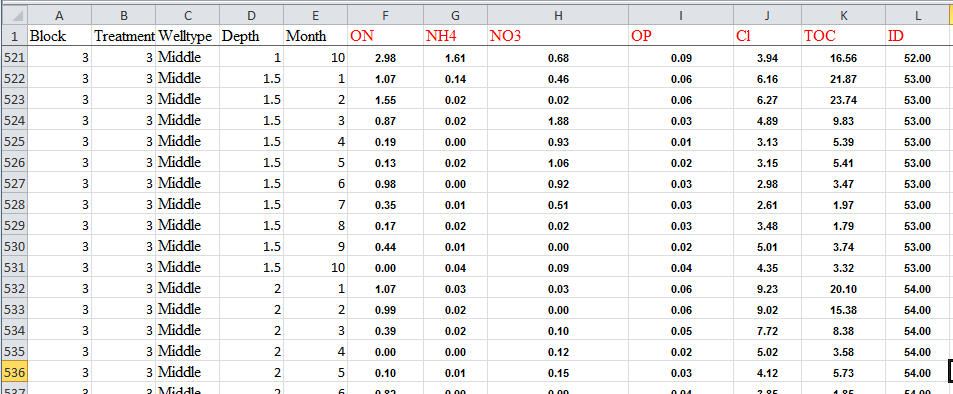
\includegraphics[scale=0.7]{spreadsheet}
\end{center}

Whether we are describing an observed population or using sampled data to draw an inference from the sample to the population, an insightful description of the data is an important step in drawing conclusions from it.  \\~\\

Good descriptive statistics enable us to make sense of the data by reducing a large set of measurements to a few summary measures that provide a good, rough picture of the original measurements.\\~\\

Summary measure used for a variable depends on its \underbar{~~~~~~~~~~~~~~~~~~~~~~~~~~~~~~~~~~~~}.\\~\\

Our goal will be to describe the variable's \underbar{~~~~~~~~~~~~~~~~~~~~~~~~~~~~~~~~~~~~}\\~\\
i.e. the \\~\\

Two major characteristics of the variable's distribution that we often describe are \underbar{~~~~~~~~~~~~~~~~~~~~~~~~~~~~~~~~~~~~}\\~\\ and \underbar{~~~~~~~~~~~~~~~~~~~~~~~~~~~~~~~~~~~~}\\~\\

We will mostly deal with quantitative variables and our focus will be on their summary measures.  However, we will briefly talk about graphs and statistics for categorical variables.\\~\\

\huge Categorical Variables \normalsize\\
Numerical measure used for categorical variable:\\~\\~\\~\\~\\
For this simple study, we can find the sample proportion for each categorical variable:\\
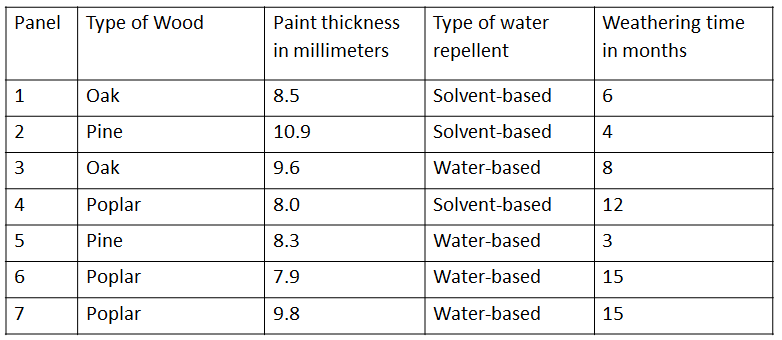
\includegraphics[scale=0.5]{paintexample}

\newpage

The main plots used are \underbar{~~~~~~~~~~~~~~~~~~~~~~~~~~~~~~~~~~~~} and  \underbar{~~~~~~~~~~~~~~~~~~~~~~~~~~~~~~~~~~~~}.\\~\\
 
\underbar{~~~~~~~~~~~~~~~~~~~~~~~~~~~~~~~~~~~~}  - use percents to display data. 
\begin{itemize}
\item Order does not matter (although should order from highest percentage to lowest)
\end{itemize}
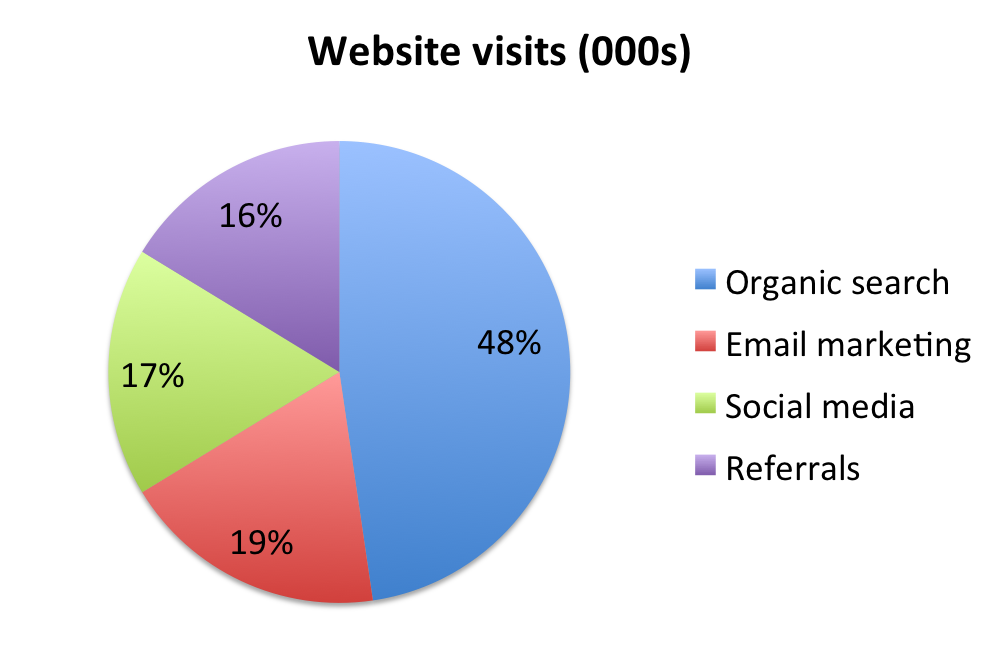
\includegraphics[scale=0.5]{piechart}\\
\underbar{~~~~~~~~~~~~~~~~~~~~~~~~~~~~~~~~~~~~}  - Categories along the x-axis.  Count, percent, or relative frequency (sample proportion) along the y-axis.  
\begin{itemize}
\item Order does not matter (although should order from highest percentage to lowest).  
\item A gap should exist between the bars.
\end{itemize}
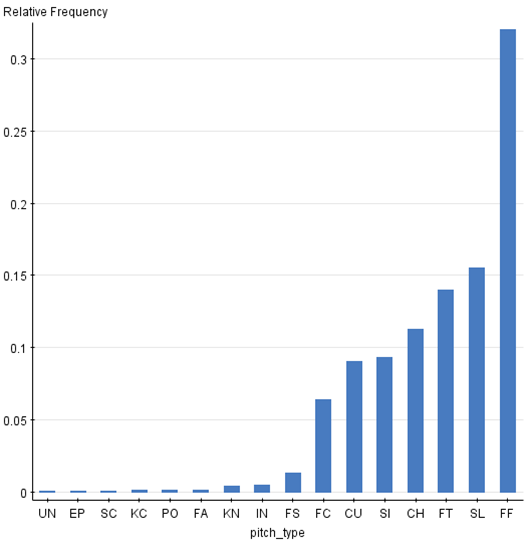
\includegraphics[scale=0.5]{bargraph}

\newpage

We might also have multiple categorical variables of interest.  In which case, a good display of the data is\\~\\
a \underbar{~~~~~~~~~~~~~~~~~~~~~~~~~~~~~~~~~~~~~~~~~~~~~~~~~~~~~}.\\~\\
Let's create one for the paint example from earlier.\\~\\~\\~\\~\\~\\~\\~\\~\\~\\~\\~\\

Book example on page 103 is nice.  \\~\\

Many other methods exist such as comparative bar charts:\\~\\
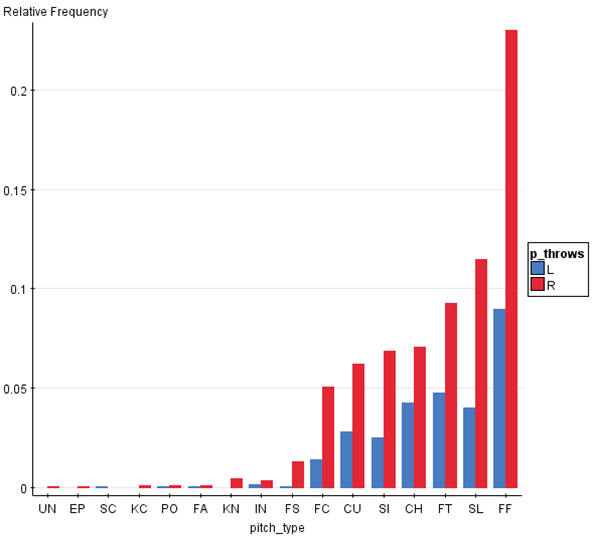
\includegraphics[scale=0.5]{bargraph2}\\~\\

\newpage
\huge Quantitative Variables \normalsize\\
We will again consider the paint example:\\
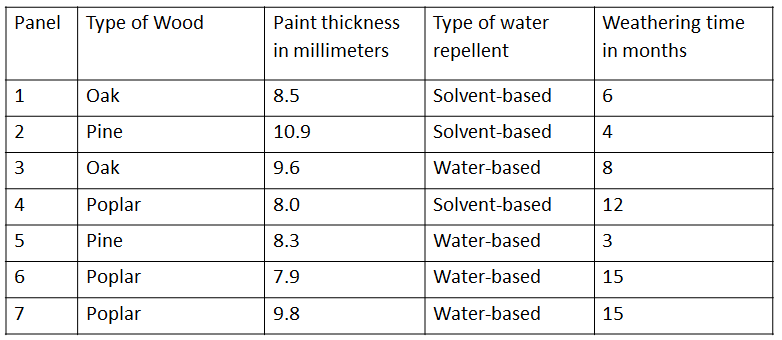
\includegraphics[scale=0.5]{paintexample}\\
Numerical measures of location:\\~\\~\\~\\~\\~\\~\\~\\~\\~\\~\\~\\~\\~\\~\\~\\~\\~\\~\\~\\
\newpage
Numerical Measures of Spread
\newpage
The main plots used are \underbar{~~~~~~~~~~~~~~~~~~~~~~~~~~~~~~~~~~~~} and  \underbar{~~~~~~~~~~~~~~~~~~~~~~~~~~~~~~~~~~~~}.\\~\\

A \underbar{~~~~~~~~~~~~~~~~~~~~~~~~~~~~~~~~~~~~} is obtained by splitting the range of the data into equal-sized bins. Then for each bin, we count the number of points that fall into each bin and that is the height of our bar (or use relative frequency - i.e. proportion in category).  
\begin{itemize}
\item Typically, an observation equal to a boundary value is put in the higher interval.
\item Bars should touch!
\item Too many classes will spread the data out, thereby not revealing the pattern.  Too few classes will lump the data.  
\item **** This is the most important graphical technique for displaying the distribution of a quantitative variable!
\end{itemize}
Ex. Ages of the winners of the best actress Academy Award in the recent 20 years (1994-2013) are: 36, 45, 49, 39, 34, 26, 25, 33, 35, 35, 28, 30, 29, 61, 32, 33, 45,29, 62 and 22\\
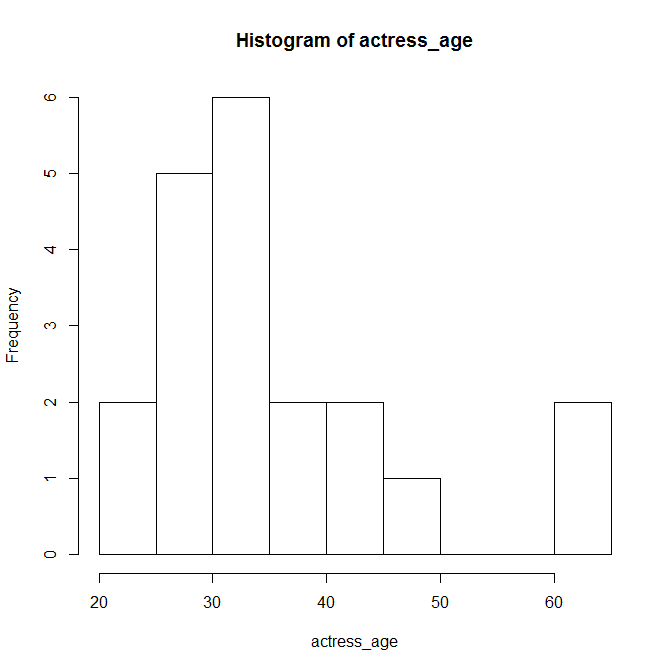
\includegraphics[scale=0.3]{oscarhist}\\

What are we looking for in a histogram?\\
\begin{itemize}
\item ~\\
\item ~\\
\item ~
\end{itemize}
\newpage

Relationship between mean and median for a histogram (note pictures use smooth curves, but same ideas hold):\\
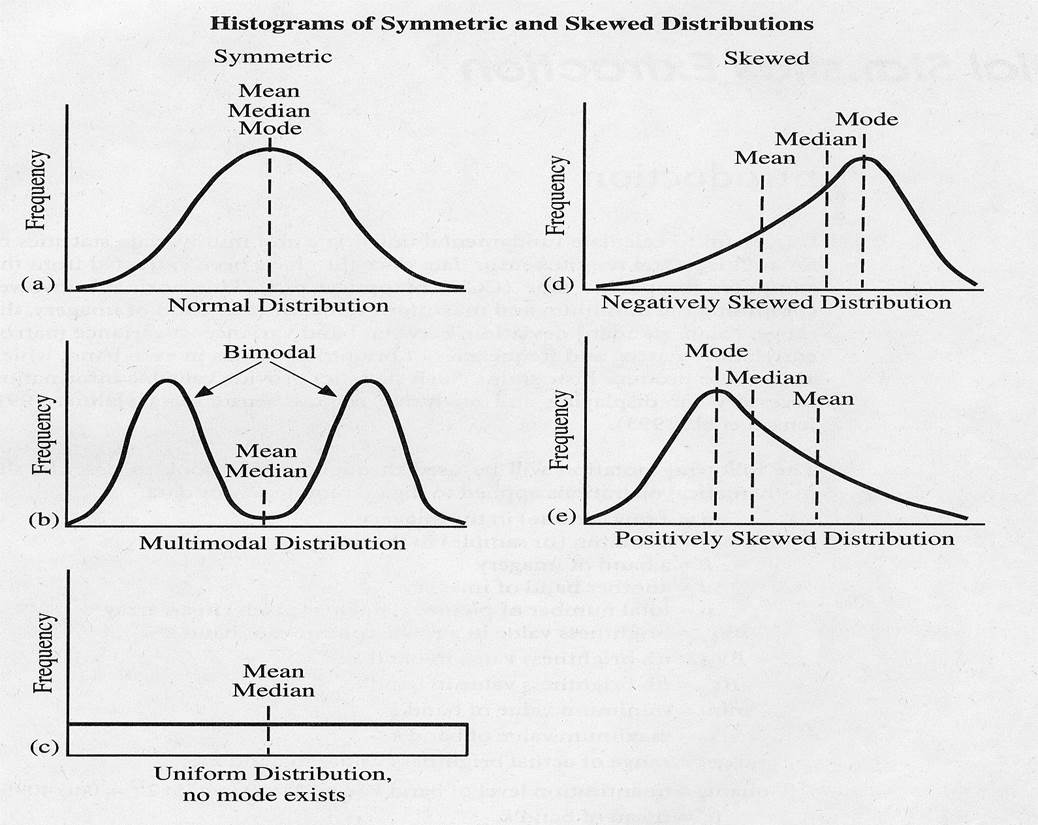
\includegraphics[scale=0.6]{meanmedianrelationship}\\


A \underbar{~~~~~~~~~~~~~~~~~~~~~~~~~~~~~~~~~~~~} displays the five number summary of the data.\\~\\
Five number summary includes:\\~\\~\\~\\

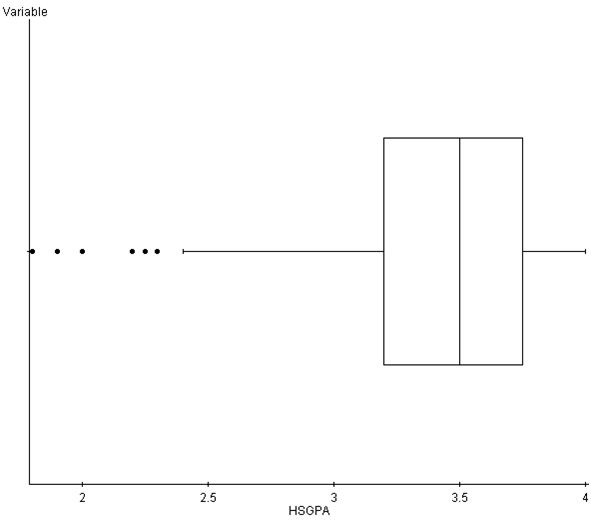
\includegraphics[scale=0.5]{boxplot2}\\
\begin{itemize}
\item Measure of center from a boxplot - \\
\item Measures of spread from a boxplot - \\~\\
\item Can tell skewness but not modality!
\end{itemize}

If we have two quantitative variables of interest, we often look at \underbar{~~~~~~~~~~~~~~~~~~~~~~~~~~~~~~~~~~~~~~~~~~~~~~~~~~~~~} \\~\\
and \underbar{~~~~~~~~~~~~~~~~~~~~~~~~~~~~~~~~~~~~~~~~~~~~~~~~~~~~~} to inspect the `linear association' between the variables (call them x and y).\\
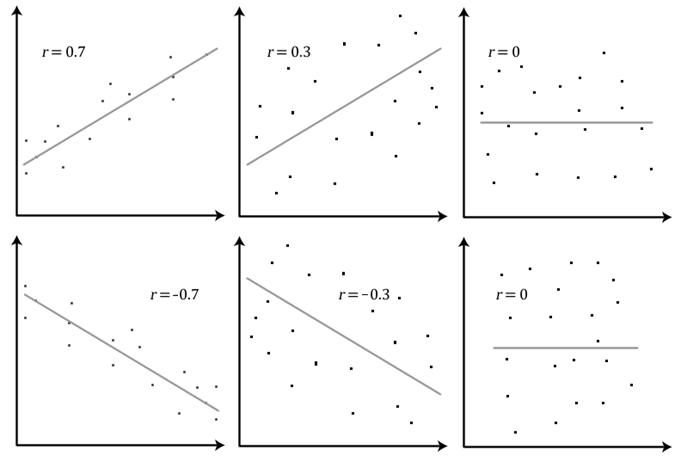
\includegraphics[scale=0.6]{scatterplots}\\
We will look at these more later in the course.\\~\\~\\
If we have a quantitative and a categorical variable, we often look at \underbar{~~~~~~~~~~~~~~~~~~~~~~~~~~~~~~~~~~~~~~~~~~~~~~~~~~~~~}.\\
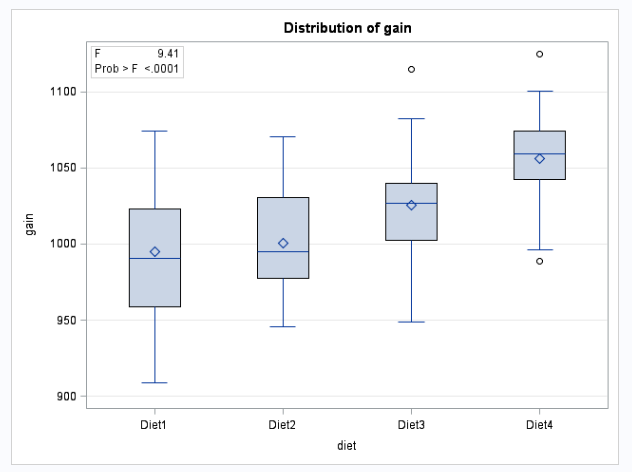
\includegraphics[scale=0.6]{ChickensBoxPlot}\\~\\
Review - \\
Numeric Summaries of Location: Mean/median/trimmed mean (quantitative), proportion (qualitative)\\
Numeric Summaries of Spread: Variance, SD, IQR, CV, Quartiles (quantitative)\\
Graphical Summaries for categorical: Bar Chart, Pie Graph\\
Graphical Summaries for quantitative: Histogram, Boxplot






